\section{Redes Estocásticas}

\subsection{Definições}
\begin{frame}{Redes Estocásticas}%
  \justifying%
  Podemos considerar também o caso em que as unidades $\mathrm{x}_{i}$ de uma rede são variáveis aleatórias.
  \\~\\
  A unidade $\mathrm{x}_{i}$ tem agora certa probabilidade $g(h_{i})$ de ser encontrado com valor $x_{i} = 1$, e probabilidade $1 - g(h_{i})$, com valor $x_{i} = 0$.
\end{frame}

\begin{frame}{Função de Ativação}%
  \justifying%
  Outra forma para a função de ativação:
  \begin{figure}[h]{}%
    \label{fig:stoc-activation}%
    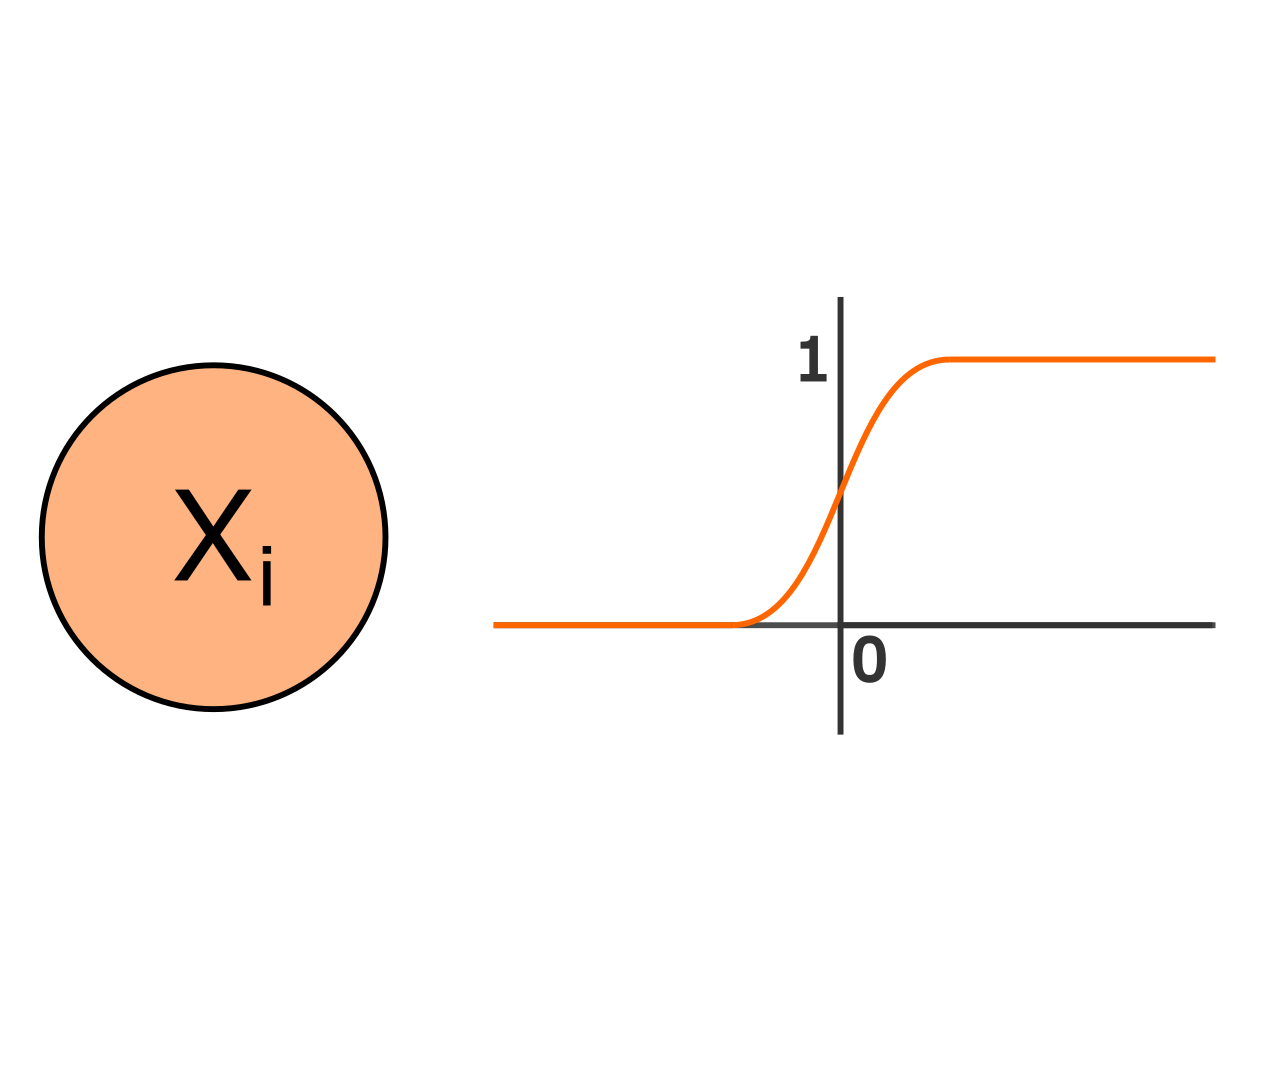
\includegraphics[scale=0.35]{images/stochastic_activation.png}
    \caption{Função de ativação no caso estocástico. Trata-se de uma função logistica, e não mais uma função degrau.}
  \end{figure}
\end{frame}

\begin{frame}{Função de Ativação}%
  \justifying%
  Função logística, ao invés de função degrau $\dots$
  \begin{equation}%
    \label{eq:stoc-logistic}
    x_{i} = g(h_{i}) = \frac{1}{1 + e^{(-\beta h_{i})}}
  \end{equation}
  \\~\\
  \begin{equation}%
    \label{eq:hi}%
    h_{i} = \sum_{j} \omega_{ij} x_{j}
  \end{equation}
\end{frame}

\begin{frame}{Temperatura -- Ruído}%
  \justifying%
  Na equação~(\ref{eq:stoc-logistic}), temos o parâmetro $\beta$, que corresponde ao inverso da temperatura $T$.
  \\~\\
  Esta temperatura não tem o mesmo significado físico, mas é usado aqui para introduzir ruído. Controlar a inclinação da função logística.
  \\~\\
  Se $\beta$ for muito grande, ou seja, temperatura muito baixa, o sistema retorna à situação determinística. A função logística passa a ser a função degrau.
  \\~\\
  Possibilidade de escapar de mínimos locais!
\end{frame}

\subsection{Esquema}
\begin{frame}{Rede Estocásticas diagrama}%
  \begin{figure}%
    \label{fig:stoc-diagram}%
    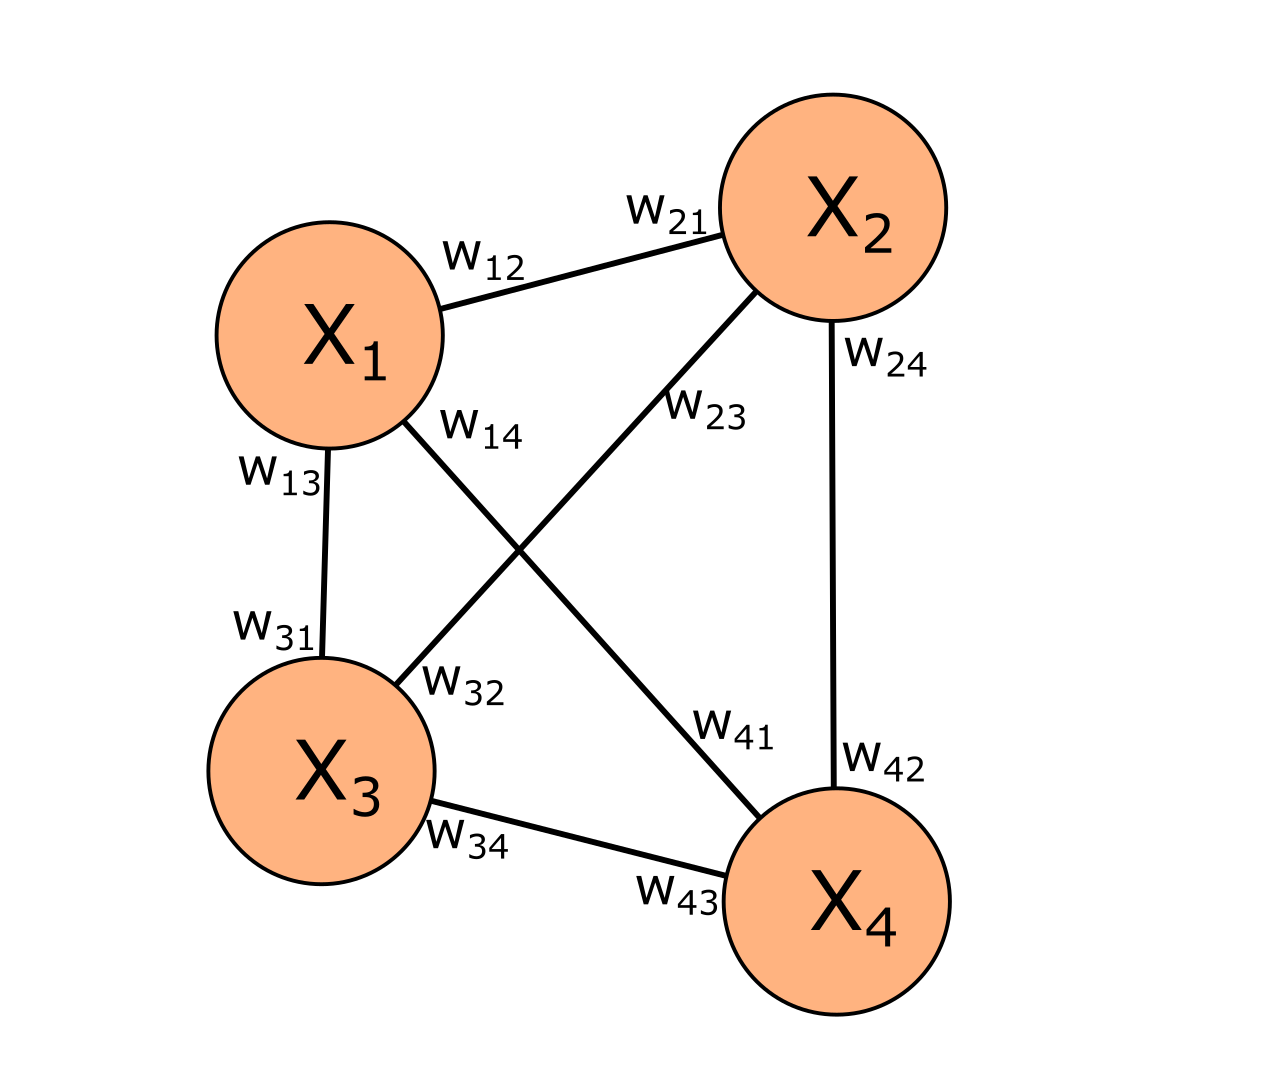
\includegraphics[scale=0.5]{images/stochastic_full.png}
    \caption{Rede estocástica com 4 unidades, e seus respectivas pesos.}
  \end{figure}
\end{frame}

\begin{frame}{Funcionamento da rede Estocástica}%
  \justifying%
  Novamente, mostramos um novo estado para a rede, por exemplo, $\mathrm{\mathbf{x}} = (1, 1, 1, 0)$.
  \\~\\
  Partimos de uma unidade aleatória para ser atualizada. Agora para determinarmos se ela está ativa ou não, pela função logistica, equação~(\ref{eq:stoc-logistic}).
\end{frame}

\begin{frame}{Funcionamento da rede Estocástica}%
  \justifying%
  Considerando que todas as unidades são atualizadas de forma aleatória, a rede vai alcançar um equilíbrio, isto é, o valor das unidades deixará de mudar. Dizemos que o sistema encontra-se estacionário.
  \\~\\
  Nesta condição, a probabilidade de encontrarmos a rede no estado em que se manteve estacionária, $\mathrm{\mathbf{x}}_{s}$, é dada pela distribuição de Boltzmann
  \begin{align}%
    \label{eq:stoc-bd}%
    P(\mathbf{x}_{s}) &= \frac{e^{-\beta H(\mathbf{x}_{s})}}{Z}, \\
    Z & = \sum_{\mathbf{u}} e^{-\beta H(\mathbf{u})}.
  \end{align}
  %A probabilidade é dada unicamente pela a energia do estado relativo a energia de todos os estados possíveis!
\end{frame}
